\chapter{Struttura}
\noindent Per il corretto funzionamento dell'applicazione, è essenziale avviare gli applicativi server e client in sequenza.\\
\\
Per avviare il server, la classe \texttt{StartServer}:
\begin{enumerate}
    \item \textit{Istanzia} il \textbf{server} principale e i due server secondari;
    \item \textit{Assegna} a ognuno di questi una \textbf{porta}, arbitrariamente 1926, 1927 e 1928;
    \item \textit{Istanzia} un \textbf{thread} per ognuno dei server.\\
        Ogni thread inizia automaticamente l’esecuzione del main-loop del server, ossia si pone in ascolto di connessioni e crea un ulteriore thread per ogni client che si connette.
\end{enumerate}
Ogni \textit{client} è gestito da un’appropriata \textit{strategia}, implementate nelle classi:
\begin{itemize}
    \item \texttt{AppointmentClientStrategy}: per il gestore degli appuntamenti;
    \item \texttt{HandlerClientStrategy}: per il gestore principale;
    \item \texttt{PosterClientStrategy}: per il gestore degli immobili.
\end{itemize}
La logica di base per la \textit{comunicazione} con il client è implementata all’interno della classe \texttt{ClientManager}, che offre funzioni di utilità per leggere o scrivere un messaggio sullo stream della socket; questa classe inoltre fornisce un oggetto per la connessione e la gestione del database attraverso \texttt{DatabaseConnectionProxy}.\\
\\
Per \textbf{avviare il programma} client, la classe \texttt{StartApplication} estende la classe \texttt{Application} e fornisce le istruzioni di configurazione per l'interfaccia e l'avvio.\\
\\
La \textbf{creazione delle \texttt{interfacce grafiche}} è definita all'interno dei file \texttt{FXML}, dove vengono specificati gli elementi che le compongono e le relative proprietà.\\ 
Ogni interfaccia è associata a una classe \texttt{Controller}, il cui compito è gestire sia l'aspetto grafico che la logica sottostante tramite codice.\\
\\
Per la \textbf{gestione dei dati} degli:
\begin{itemize}
    \item \textbf{Immobili:} è stata realizzata la classe \texttt{House}, i cui oggetti sono creati ed affidati a una gerarchia di classi che segue il pattern "Builder";
    \item \textbf{Appuntamenti:} è stata implementata la classe \texttt{Appointment};
    \item \textbf{Utenti loggati:} è stata sviluppata la classe \texttt{User}.
\end{itemize}

\section{Pattern}

\noindent Per l'implementazione dei server, sono stati adottati due \textbf{design pattern}, uno  comportamentale (\texttt{STRATEGY}) ed uno strutturale (\texttt{PROXY}).\\
Il primo implementa il caricamento on-demand del database per questioni di performance mentre l'altro, tramite scambio di messaggi in JSON, implementa la selezione degli algoritmi fini allo smistamento dei server ausiliari da parte dell'handler.

\subsection{Proxy}

\noindent È un pattern structural che consente di fornire un sostituto o un placeholder per un altro oggetto. Il proxy controlla l'accesso all'oggetto originale, consentendo di eseguire qualcosa prima o dopo che la richiesta sia arrivata all'oggetto originale.

\subsubsection{Utilizzo pratico}
\noindent Nel nostro caso, è stato utilizzato un "Virtual Proxy" per la connessione al database nei server secondari. Questo approccio ci permette di creare la connessione solo quando è effettivamente necessaria (on-demand), evitando così il costo di una connessione costante.

\begin{figure}[htbp]
    \centering
    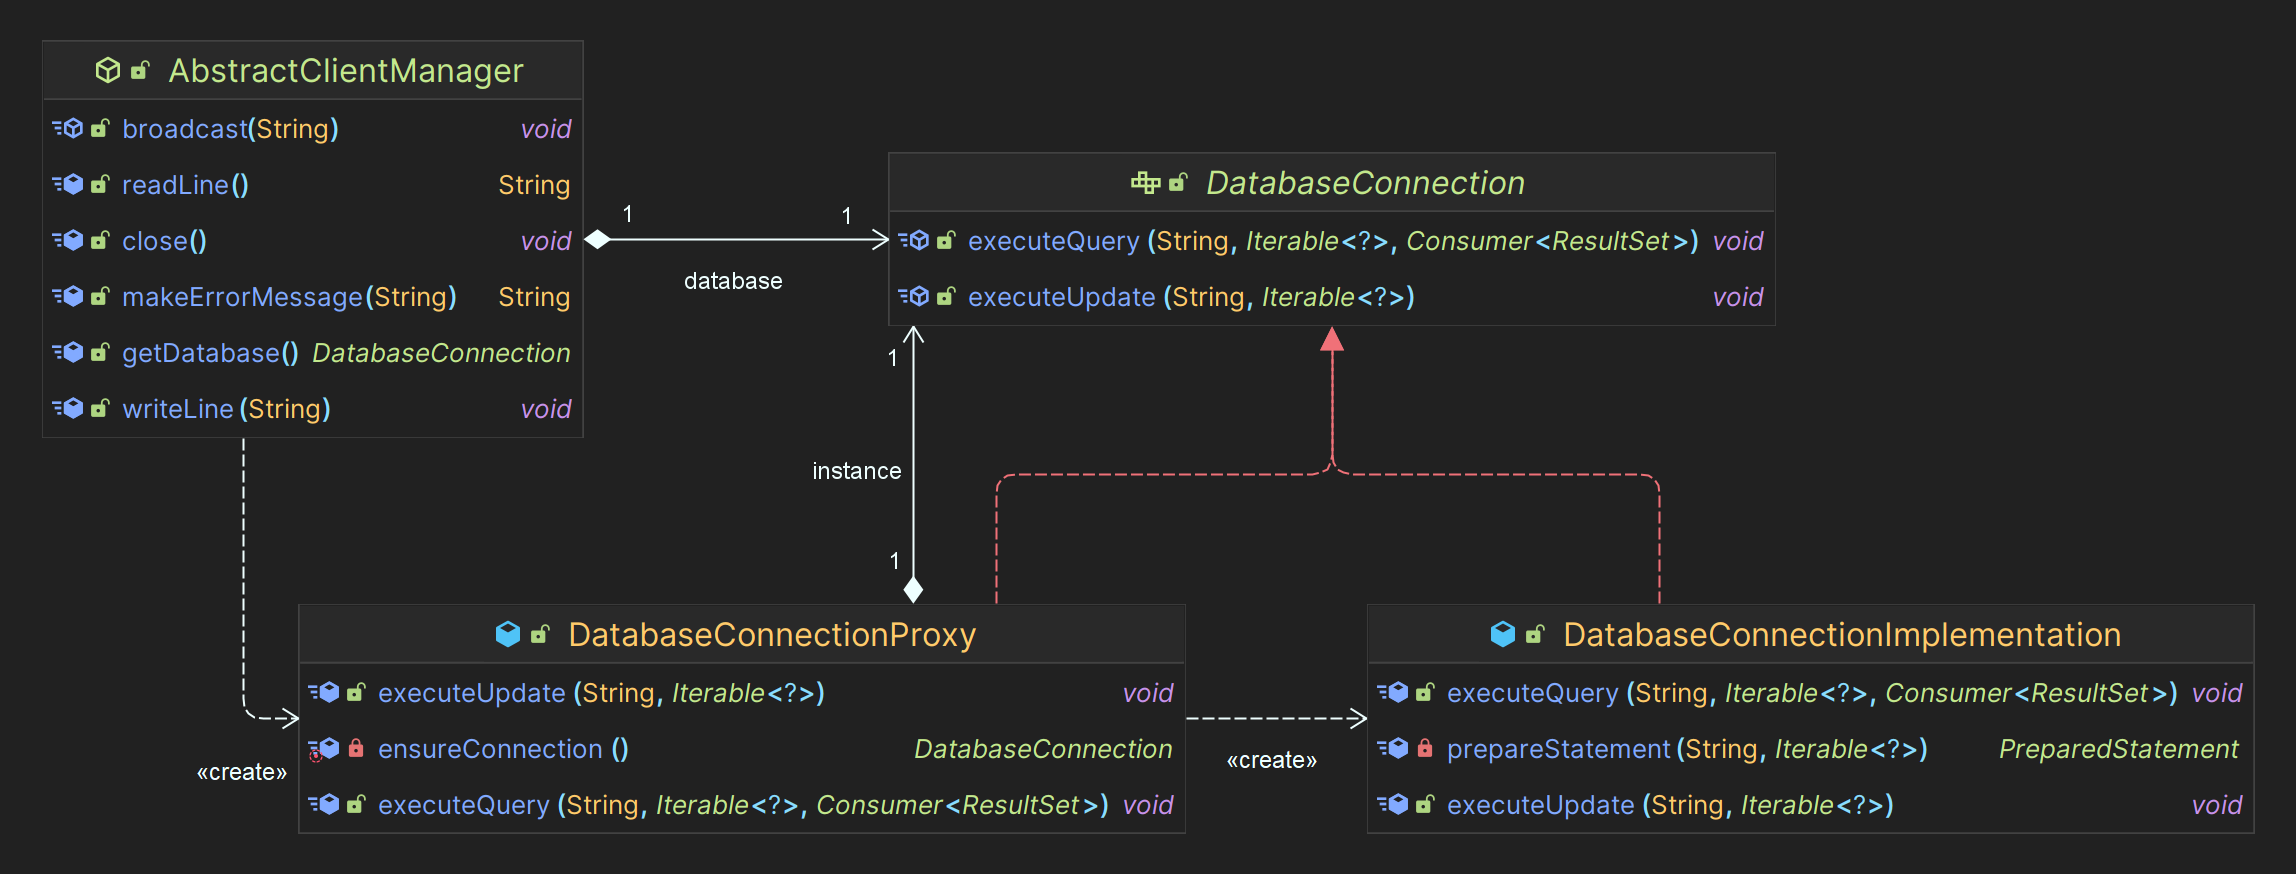
\includegraphics[width=\textwidth,height=\textheight,keepaspectratio]{ProxyUMLdetailed.png}
    \caption{Struttura Proxy pattern implementato nel SW con metodi}
\end{figure}

\subsection{Strategy}

\noindent Questo pattern behavioural definisce una famiglia di algoritmi, incapsulandoli e rendendoli intercambiabili. Si usa quando si ha necessità di modificare dinamicamente gli algoritmi utilizzati dall’applicazione.\\
\textit{N.B.:} L’algoritmo cambia indipendentemente dai client che lo usano

\subsubsection{Utilizzo pratico}
\noindent Nel nostro caso, questo pattern è stato utilizzato per implementare facilmente la gestione dei  comportamenti dei vari server, questi forniscono funzionalità diverse e gestiscono messaggi diversi ma, alla base delle loro funzionalità c’è sempre lo stesso principio: lo scambio di messaggi.

\begin{figure}[htbp]
    \centering
    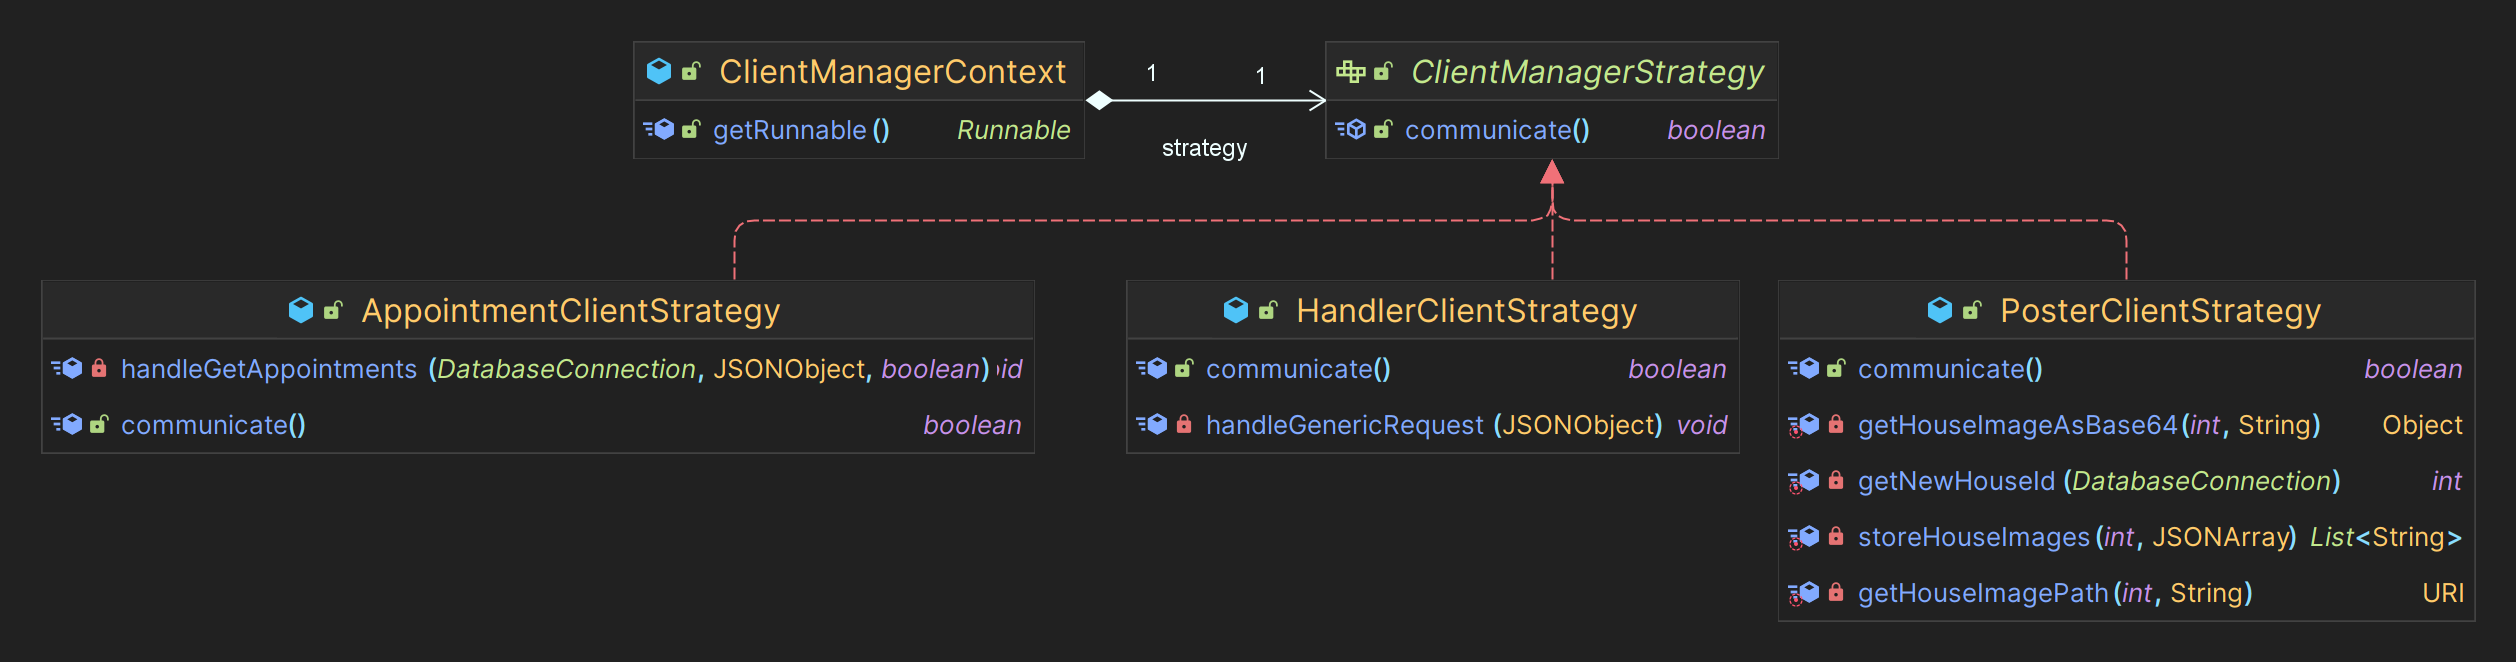
\includegraphics[width=\textwidth,height=\textheight,keepaspectratio]{StrategyUMLdetailed.png}
    \caption{Struttura Strategy pattern implementato nel SW con metodi}
\end{figure}